% begin module curve-sketching-guidelines
\begin{frame}
\frametitle{Guidelines for Sketching a Curve}
Consider the following things when asked to sketch a curve.  Not every one of these guidelines is relevant to every function.
\begin{enumerate}
\item  Domain
\item  Intercepts
\item  Symmetry
\item  Asymptotes
\item  Intervals of increase or decrease
\item  Local maxima and minima
\item  Concavity and points of inflection
%\item  Sketch the curve
\end{enumerate}
\end{frame}

\begin{frame}[t]
\begin{enumerate}
\item  Domain
\end{enumerate}
\begin{itemize}
\item  Find the domain of the function.  
\item  Remember the two restrictions: no dividing by $0$, and no taking the even root of a negative number.
\end{itemize}
\end{frame}


\begin{frame}[t]
\begin{enumerate}
\setcounter{enumi}{1}
\item  Intercepts
\end{enumerate}
\begin{itemize}
\item  Find the intercepts of the function.
\item  $f(0)$ is the $y$-intercept.
\item  To find the $x$-intercepts, set $y = 0$ and solve for $x$.
\item  You can sometimes skip this step if the equation is too difficult to solve.
\end{itemize}
\end{frame}


\begin{frame}[t]
\begin{enumerate}
\setcounter{enumi}{2}
\item  Symmetry
\end{enumerate}
\begin{itemize}
\item<1-| alert@2>  \alert<handout:1| 0>{If $f(-x) = f(x)$ for all $x$, then $f$ is even.}
\item<1-| alert@3>  \alert<handout:2| 0>{If $f(-x) = -f(x)$ for all $x$, then $f$ is odd.}
\item<1-| alert@4>  \alert<handout:3| 0>{If there is some number $p$ such that $f(a+p) = f(a)$ for all $a$, then $f$ is called periodic.  The smallest such $p$ is called its period.}
\end{itemize}
\begin{center}
\ \only<handout:1| -2>{%
\uncover<2>{%
\ 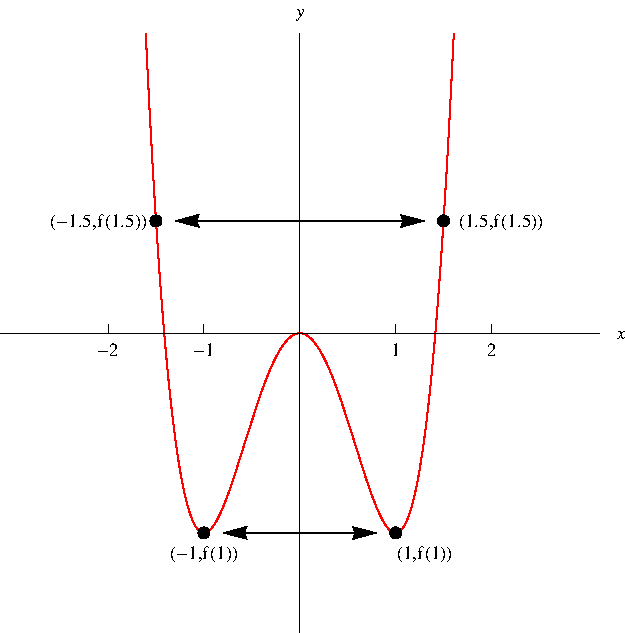
\includegraphics[height=5cm]{curve-sketching/pictures/01-01-even.pdf}%
}}%
\only<handout:2| 3>{%
\ 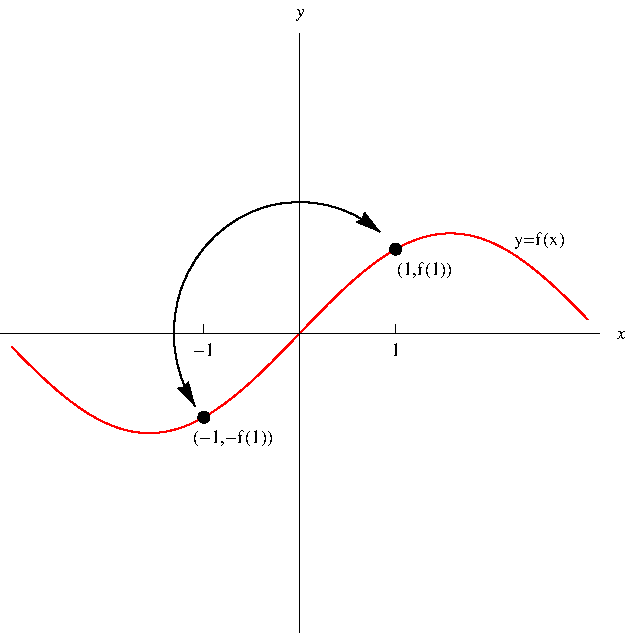
\includegraphics[height=5cm]{curve-sketching/pictures/01-01-odd.pdf}%
}%
\only<handout:3| 4->{%
\ 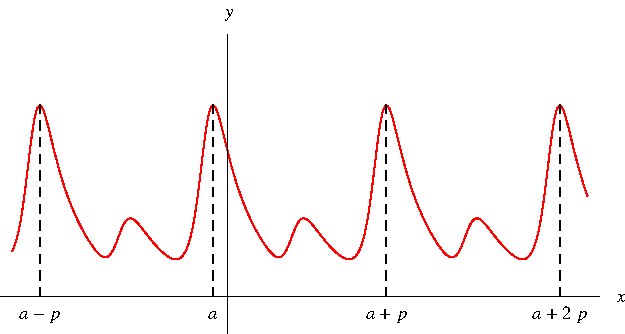
\includegraphics[height=5cm]{curve-sketching/pictures/04-05-periodic.pdf}%
}
\end{center}
\end{frame}


\begin{frame}[t]
\begin{enumerate}
\setcounter{enumi}{3}
\item  Asymptotes
\end{enumerate}
\begin{itemize}
\item  \textbf{Horizontal asymptotes} can be found by finding $\lim_{x\to\infty} f(x)$ and $\lim_{x\to -\infty} f(x)$.
\item  If either of these equals a number $L$, then $y = L$ is a horizontal asymptote of $f$.  
\item  If neither limit is finite, there is no horizontal asymptote.
\item  The line $x = a$ is a \textbf{Vertical asymptote} of $f$ if any of the following is true
\end{itemize}
\[
\begin{array}{ll}
\displaystyle \lim_{x\to a^+}f(x) = \infty &%
\displaystyle \lim_{x\to a^-}f(x) = \infty \\%
\displaystyle \lim_{x\to a^+}f(x) = -\infty &%
\displaystyle \lim_{x\to a^-}f(x) = -\infty %
\end{array}
\]
\begin{itemize}
\item  We will discuss \textbf{slant asymptotes} later in section 4.5.
\end{itemize}
\end{frame}


\begin{frame}[t]
\begin{enumerate}
\setcounter{enumi}{4}
\item  Intervals of increase or decrease
\end{enumerate}
\begin{itemize}
\item  To find intervals of increase or decrease, use the increasing/decreasing test.
\item  Compute $f'$.
\item  Find where $f'$ is positive or negative.
\item  Where $f'$ is positive, $f$ is increasing.
\item  Where $f'$ is negative, $f$ is decreasing.
\end{itemize}
\end{frame}




\begin{frame}[t]
\begin{enumerate}
\setcounter{enumi}{5}
\item  Local maxima and minima
\end{enumerate}
\begin{itemize}
\item  Find the critical numbers of $f$ (the numbers $c$ where $f'(c)$ doesn't exist or $f'(c) = 0$).
\item  Use the First Derivative Test on each of these numbers:
\item  If $f'$ changes from positive to negative at a critical number $c$, then $c$ is a local maximum.
\item  If $f'$ changes from negative to positive at a critical number $c$, then $c$ is a local minimum.
\item  If $f'$ doesn't change sign at a critical number $c$, then $c$ is neither a local maximum nor a local minimum.
\end{itemize}
\end{frame}



\begin{frame}[t]
\begin{enumerate}
\setcounter{enumi}{6}
\item  Concavity and points of inflection
\end{enumerate}
\begin{itemize}
\item  To find inflection points and intervals of concavity, use the concavity test.
\item  Compute $f''$.
\item  Find where $f''$ is positive or negative.
\item  Where $f''$ is positive, $f$ is concave up.
\item  Where $f''$ is negative, $f$ is concave down.
\item  Inflection points occur when $f''$ changes signs.
\end{itemize}
\end{frame}
% end module curve-sketching-guidelines
